\documentclass{article}

\usepackage{amsthm}

% !TeX TXS-program:compile = txs:///pdflatex/[--shell-escape]

\usepackage{amsfonts}
\usepackage{amsmath}
\usepackage{amssymb}
\usepackage{fullpage}
\usepackage[usenames]{color}
\usepackage{hyperref}
  \hypersetup{
    colorlinks = true,
    urlcolor = blue,       % color of external links using \href
    linkcolor= blue,       % color of internal links 
    citecolor= blue,       % color of links to bibliography
    filecolor= blue,        % color of file links
    }
    
\usepackage{listings}
\usepackage{minted}
\usepackage{graphicx}

\definecolor{dkgreen}{rgb}{0,0.6,0}
\definecolor{gray}{rgb}{0.5,0.5,0.5}
\definecolor{mauve}{rgb}{0.58,0,0.82}

\lstset{frame=tb,
  language=haskell,
  aboveskip=3mm,
  belowskip=3mm,
  showstringspaces=false,
  columns=flexible,
  basicstyle={\small\ttfamily},
  numbers=none,
  numberstyle=\tiny\color{gray},
  keywordstyle=\color{blue},
  commentstyle=\color{dkgreen},
  stringstyle=\color{mauve},
  breaklines=true,
  breakatwhitespace=true,
  tabsize=3
}

\theoremstyle{theorem} 
  \newtheorem{theorem}{Theorem}[section]
  \newtheorem{corollary}[theorem]{Corollary}
  \newtheorem{lemma}[theorem]{Lemma}
  \newtheorem{proposition}[theorem]{Proposition}
\theoremstyle{definition}
  \newtheorem{definition}[theorem]{Definition}
  \newtheorem{example}[theorem]{Example}
\theoremstyle{remark}    
  \newtheorem{remark}[theorem]{Remark}


\title{CPSC-354 Report}
\author{Natalie Huante  \\ Chapman University}

\date{\today}

\begin{document}

\maketitle

\begin{abstract}
Short  summary of purpose and content.  
\end{abstract}

\tableofcontents

\section{Introduction}\label{intro}

\section{Homework}\label{homework}

This section contains solutions to homework. 

\subsection{Week 1}

The homework for Week 1 is dedicated to allow myself the opportunity to get familiar with LaTeX as well as review the model of equational reasoning. 
In this lesson, we used the Fibonacci Sequence as an example of this but we will use the function of Greatest Common Divisor for the assignment.
In terms of familiarity with LaTeX, I do have experience through the Algorithm Analysis report from the previous 
semester, however, this serves as a way to remind myself of the language. \\


For context, the definition the GCD function is as follows:
\begin{verbatim}
gcd(a,b): 
Input: Two whole numbers (integers) called a and b, both greater than 0.
(1) if a>b then replace a by a-b and go to (1).
(2) if b>a then replace b by b-a and go to (1).
Output: a
\end{verbatim}

Now, I will write out the full computation of gcd(9,33) below:

\begin{align*}
  gcd(9,33) & = gcd(9,24)\\
            & = gcd(9,15)\\
            & = gcd(9,6)\\
            & = gcd(3,6)\\
            & = gcd(3,3)\\
            & = 3
\end{align*}

As you can see above, the basis of the function is to iteratively decrement a and b until you reach a point at which you can no longer
decrement them by the definition given. 

\subsection{Week 2}
For this week's homework we wil take a look and practice based on our discussion of the Towers of Hanoi problem. To solve the Towers of Hanoi one must move all the rings
from the left-most tower to the right-most tower. However, discs can only be placed on other discs larger than themselves. Therefore, we have to logically think about the 
order in which we move them as well as how we can most efficiently do so (the least amount of moves). I have included a visual representation of what this problem looks like: 
\begin{center}
  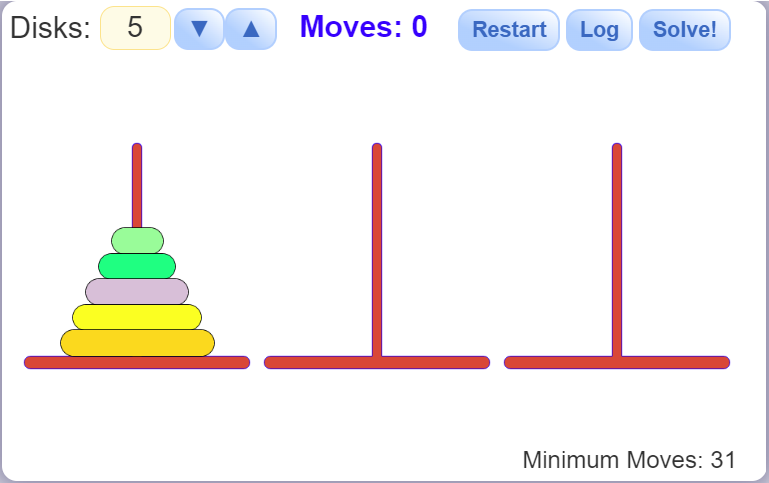
\includegraphics[scale=0.7]{towersOfHanoi_visual.png}
\end{center}

In our class discussion, we established a set of rules in order to then discuss how to represent our functions in code. Below I include both rules as well as repeat some notes on notation 
in order to allow for some context on the second half of this assignment.
\begin{minted}{haskell}
  hanoi 1 x y = move x y 

  hanoi (n+1) x y = 
    hanoi n x (other x y)
    move x y 
    hanoi n (other x y) y
\end{minted}
\begin{itemize}
  \item read \mintinline{haskell}{hanoi n x y} as "move tower of n disks from x to y"
  \item think about how to move a tower of n+1 disks assuming we already know how to move a tower of n disks 
  \item \mintinline{haskell}{hanoi n x y} is a function that takes three arguments: a number n (the number of disks), a number x (encoding the place where the tower is, a number y (encoding the place
  where the tower should go))
  \item \mintinline{haskell}{move x y} is afunction that moves one disk (the topmost disk) from x to y 
  \item \mintinline{haskell}{other x y} denotes the third place which is neither x nor y 
\end{itemize}

Now having laid down some rules for our discussion, we observed that the nature of the Towers of Hanoi problem is recursive given that in order to solve a tower of 4 disks we must first solve 
it with 3 disks and then that requires we solve it for 2 disks and so on. In class we observed the 5 disk tower solution of \mintinline{haskell}{hanoi 5 0 2}. For this assignment, I will write out the 
implementation of this function to cement what we learned about its recursion and logic. 
\begin{minted}{haskell}
  hanoi 5 0 2
    hanoi 4 0 1
      hanoi 3 0 2
        hanoi 2 0 1
          hanoi 1 0 2 = move 0 2
          move 0 1
          hanoi 1 2 1 = move 2 1
        move 0 2
        hanoi 2 1 2 
          hanoi 1 1 0 = move 1 0 
          move 1 2
          hanoi 1 0 2 = move 0 2
      move 0 1
      hanoi 3 2 1 
        hanoi 2 2 0
          hanoi 1 2 1 = move 2 1 
          move 2 0
          hanoi 1 1 0 = move 1 0
        move 2 1
        hanoi 2 0 1
          hanoi 1 0 2 = move 0 2
          move 0 1
          hanoi 1 2 1 = move 2 1
    move 0 2
    hanoi 4 1 2
      hanoi 3 1 0
        hanoi 2 1 2
          hanoi 1 1 0 = move 1 0
          move 1 2
          hanoi 1 0 2 = move 0 2
        move 1 0
        hanoi 2 2 0
          hanoi 1 2 1 = move 2 1
          move 2 0
          hanoi 1 1 0 = move 1 0
      move 1 2
      hanoi 3 0 2
        hanoi 2 0 1
          hanoi 1 0 2 = move 0 2
          move 0 1
          hanoi 1 2 1 = move 2 1
        move 0 2
        hanoi 2 1 2
          hanoi 1 1 0 = move 1 0 
          move 1 2
          hanoi 1 0 2 = move 0 2
\end{minted}

As we can see this is a very lengthy program that relies on its recursive nature to solve the hanoi problem. Now, if we extract from this execution the moves that solve the puzzle (in their right order), we will see that there are 31 moves for the 5-disk tower 
that will solve the problem most efficiently. I say that these are the steps that actually solve the problem since they are the ones that will prompt moving a disk from one tower to another. I will rewrite the steps again below: 
\begin{minted}{haskell}
  move 0 2
  move 0 1
  move 2 1
  move 0 2
  move 1 0
  move 1 2
  move 0 2
  move 0 1 
  move 2 1
  move 2 0
  move 1 0
  move 2 1
  move 0 2
  move 0 1
  move 2 1
  move 0 2
  move 1 0
  move 1 2
  move 0 2
  move 1 0
  move 2 1
  move 2 0
  move 1 0
  move 1 2
  move 0 2
  move 0 1
  move 2 1
  move 0 2
  move 1 0
  move 1 2
  move 0 2
\end{minted}

Now that we have written out the exection, we can also see that the word \mintinline{haskell}{hanoi} appear many times in the computation. I observed the number of occurrences and recorded them in the below table. By looking at the table, we can notice that the
number of occurrences can actually be represented as a formula, for they increase in the same intervals exponentially. Therefore, we can say that with n disks, the number of times the word \mintinline{haskell}{hanoi} appears in the computation is \(2^n - 1\). 
\begin{center}
  \begin{tabular}{|c c|}
    \hline
    n disks & num of hanoi \\
    \hline 
    1 & 1 \\
    \hline 
    2 & 3 \\
    \hline 
    3 & 7 \\
    \hline 
    4 & 15 \\
    \hline 
    5 & 31 \\
    \hline
  \end{tabular}
\end{center}

\subsection{Week 3}
In this week's homework, we are reviewing parsing and context-free grammars. The idea of parsing is immportant to understand as we need it to translate concrete syntax (what we see as more human-readable) into abstract syntax (what a computer will see as more readble). 
In class, we focused on processing abstract syntax in a 2-dimensional view, or what resembles a tree. A context-free grammar is a set of rules that defines a language. One of the examples we used, and the one we will use for the following problems, is a context-free grammar that 
defines arithmetic expressions. In other words, a string is considered to be part of the language defined if it can be dervied from the rules below.
\begin{minted}{haskell}
  Exp -> Exp '+' Exp1
  Exp1 -> Exp1 '*' Exp2
  Exp2 -> Integer 
  Exp2 -> '(' Exp ')'
  Exp -> Exp1
  Exp1 -> Exp2
\end{minted}
Now that we have the rules above, I will write out the derivation trees (aka parse trees or conccrete syntax trees) for the following strings. Note that I numbered the rules above and wrote, in blue, the number of the rule used in each step. The integer definition is implied here so there is no 
number next to those translations. 
\begin{itemize}
  \item 2+1
  \item 1+2*3
  \item 1+(2*3)
  \item (1+2)*3
  \item 1+2*3+4*5+6
\end{itemize}

\begin{center}
  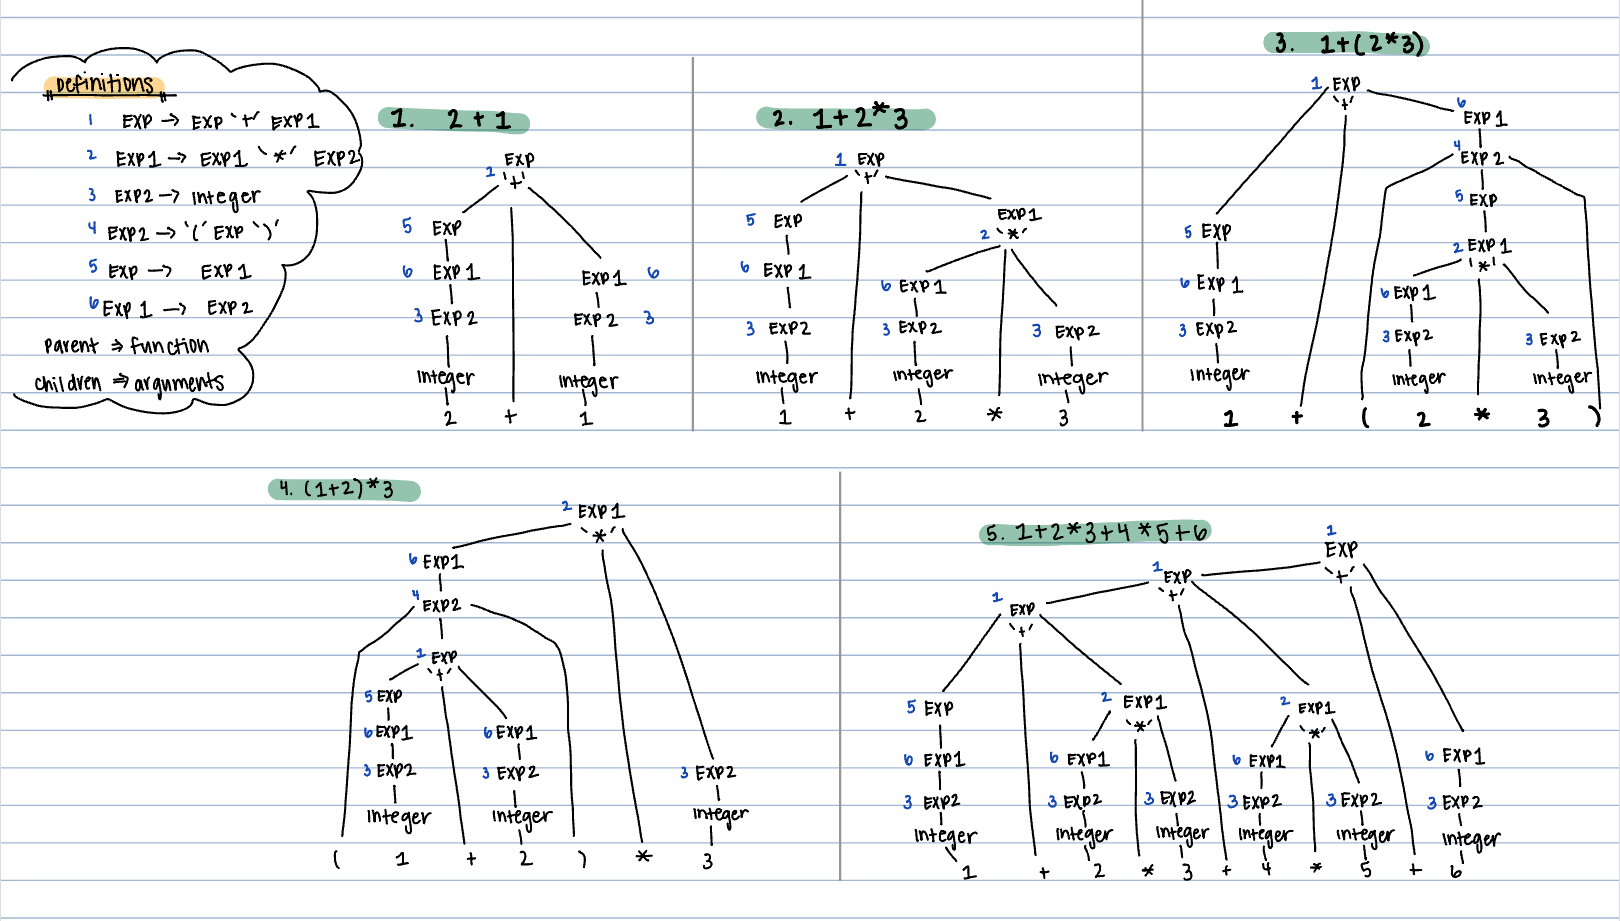
\includegraphics[scale=0.3]{parsing_arithmetic.jpg}
\end{center}


Now that we have covered what the parsing process looks like, we can think bigger. In other words, we can think of a parser that will automatically translate concrete syntax into abstract syntax. Looking at out lesson, we do not attempt to create this type of parser ourselves, but rather 
used a parser generator. In this case, we will input a context-free grammer (like the one above) and the generator will output a parser.

First, I installed the parser generator BNFC, which proved to be a feat of its own. After multiple error messages and researching quests, I was able to successfully download the generator as well as the necessary libraries (alex, happy, etc.). The first commands I used are those described in the 
lecture: 
\begin{minted}{haskell}
  bnfc -m -haskell numbers.cf
  make
  echo "1+2*3" | ./TestNumbers
\end{minted}
This generated some files and then gave me the following output: 
\begin{center}
  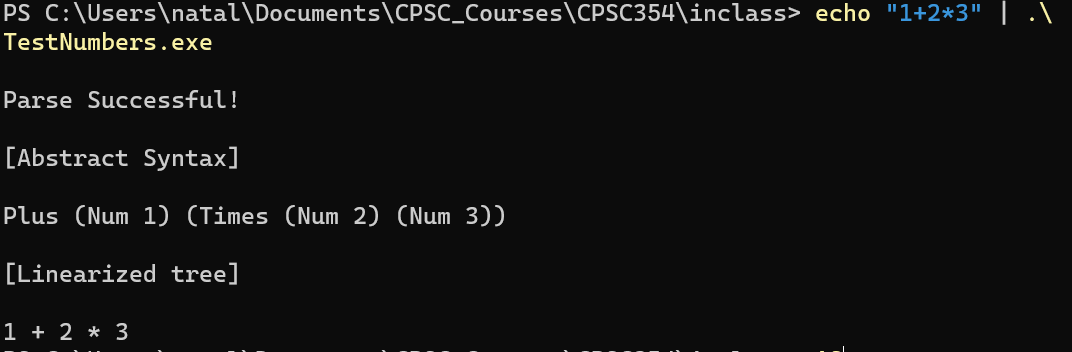
\includegraphics[width=15cm]{bnfc_intro_example.png}
\end{center}

Having run the example successfully, I will now show the outputs for the following given strings: **You will note that these are the same exercises I translated by hand above**
\begin{center}
  2 + 1 \\
  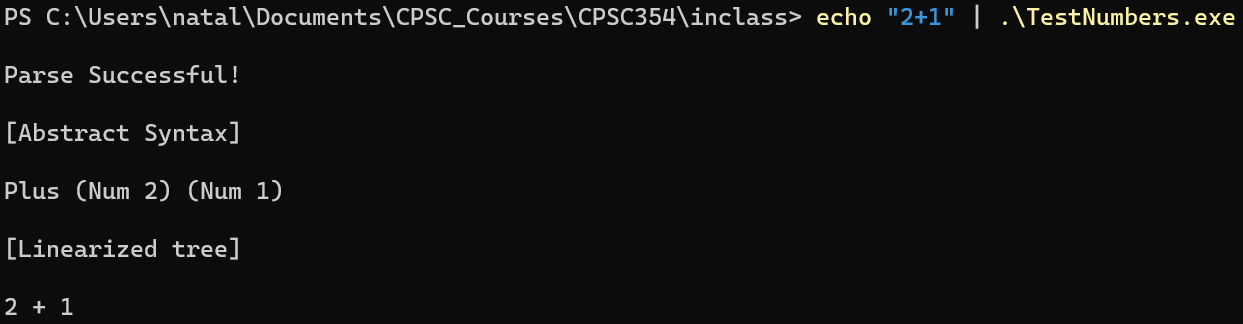
\includegraphics[width=15cm]{bnfc_exercise1a.png}

  1 + 2 * 3\\
  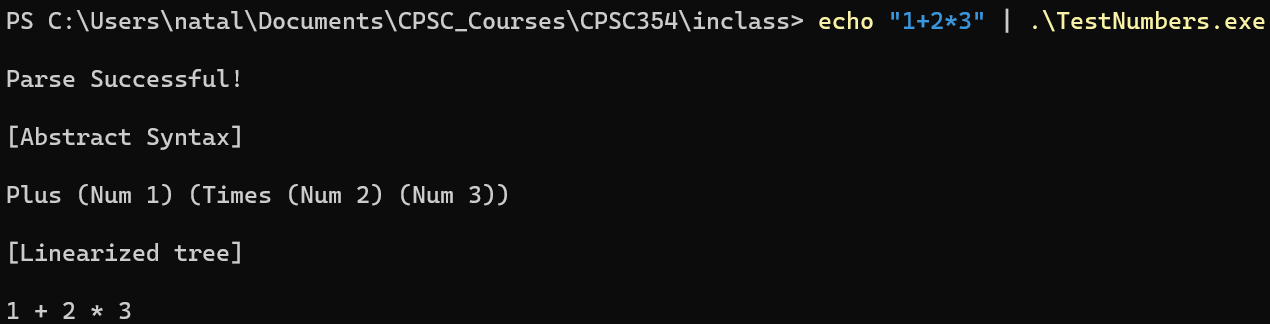
\includegraphics[width=15cm]{bnfc_exercise1b.png}

  1 + ( 2 * 3 )\\
  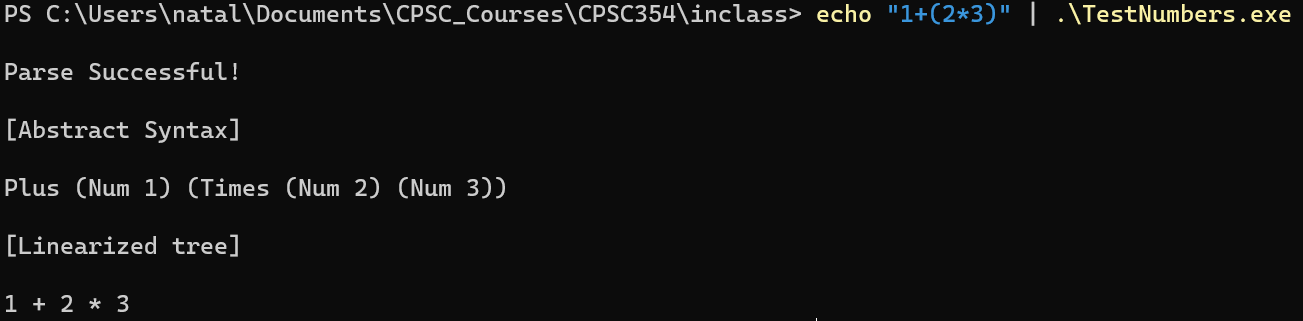
\includegraphics[width=15cm]{bnfc_exercise1c.png}

  ( 1 + 2 ) * 3\\
  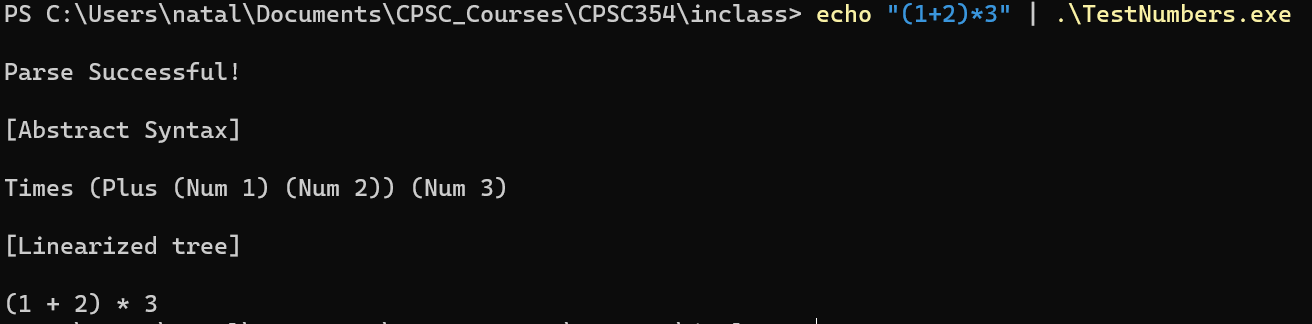
\includegraphics[width=15cm]{bnfc_exercise1d.png}

  1 + 2 * 3 + 4 * 5 + 6\\
  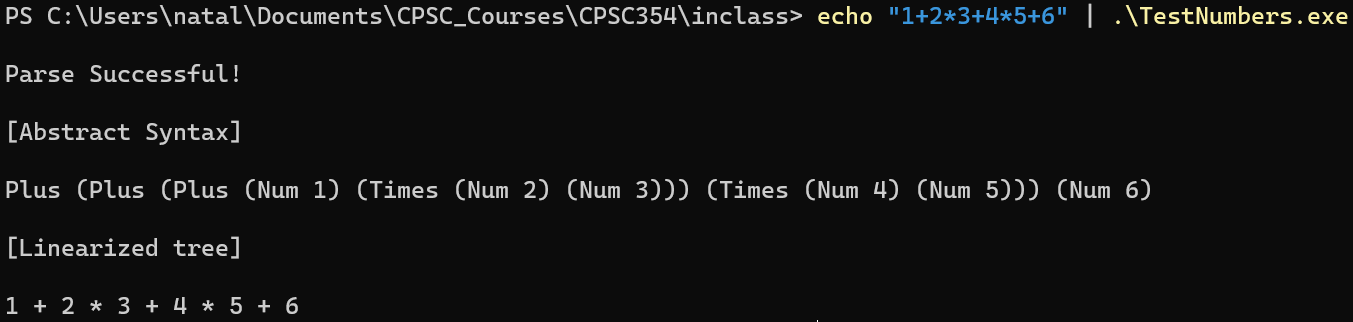
\includegraphics[width=15cm]{bnfc_exercise1e.png}
\end{center}


We can also look at the how the use of paranthesis affects the output. Here we will compare the output between 
\begin{itemize}
  \item 1+2+3
  \item (1+2)+3
  \item 1+(2+3)
\end{itemize}
\begin{center}
  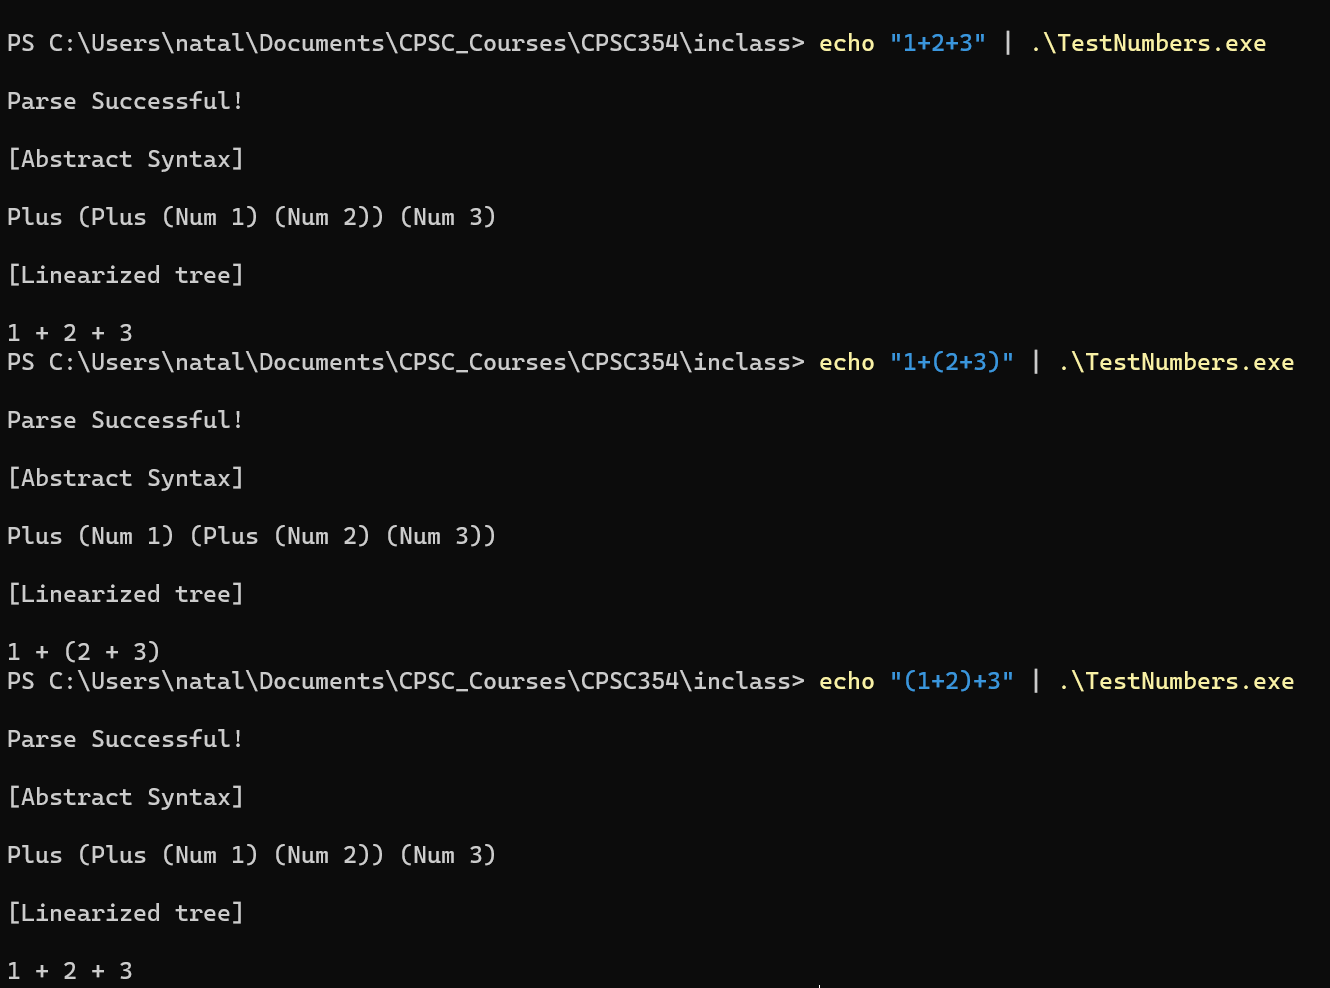
\includegraphics[width=15cm]{bnfc_exercise1f.png}
\end{center}
As you can see, the abstract syntax outputted differs depending on where or if the paranthesis are placed in the expression. The first and last output do yield the same result, implying 
that if the parser is not given any paranthesis, it will prioritize executing from left to right. In this case, the 1 and the 2 are added together first. Therefore, when the 2 and the 3 are 
placed in paranthesis, the abstract syntax changes as the order in which the addition functions are executed also changes. Overall, this homework focused on practicing with and establishing the BNFC 
environment as well as understanding how to convert concrete syntax into abstract syntax. \\

\subsection{Week 4}
This week's homework builds upon the last assignment and focuses on understanding lambda calculus. Using the layout of the previous interpreter for addition and multiplication, I first had to 
modify the definitions and interpreter to read lambda calculus. The first step of the homework was to "use bnfc and the grammar of lambda-calculus [given] to create a parser for lambda-calculus expressions." 
I include the definition provided below: 
\begin{minted}{haskell}
  Abs.   Exp ::= "\\" Ident "." Exp ;  
  App.   Exp ::= Exp Exp1 ; 
  Var.   Exp1 ::= Ident ;

  coercions Exp 1 ;
\end{minted}


Having generating a parser succesfully, I will now move on to the next section. Here, we will use the bnfc parser to write out the abstract syntax trees (in 2-dimensional notation) for 8 expressions. The first photo 
shows the 2-dimensional trees and the second code section shows the generated linearized abstract syntax tree I got from the bnfc-generated parser: 
\begin{center}
  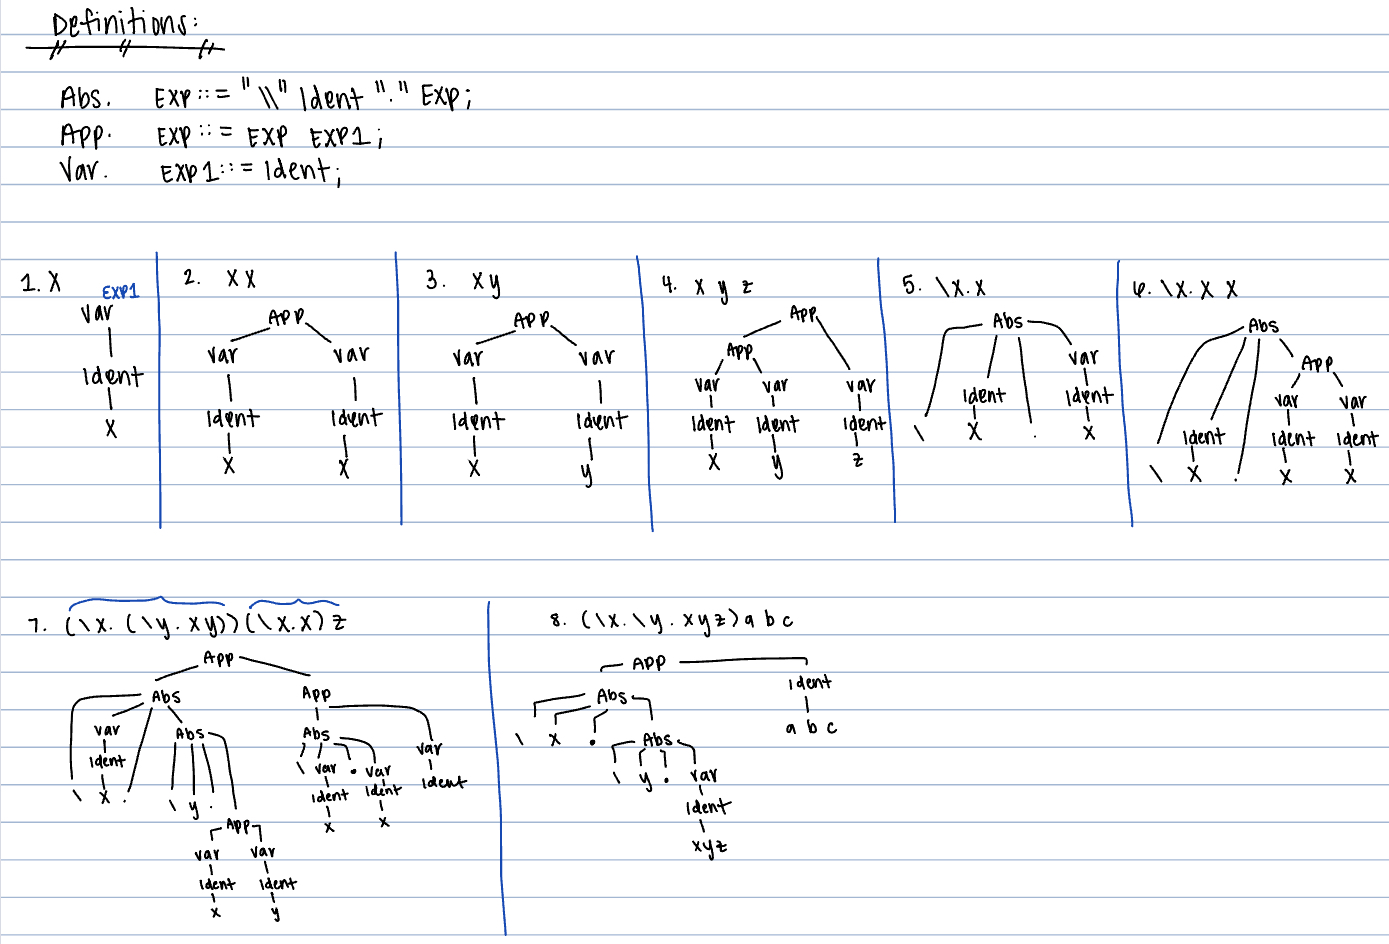
\includegraphics[width=15cm]{Week4hw_Trees.jpg}
  \begin{minted}{haskell}
    x linearized: x
    x x linearized: x x
    x y linearized: x y
    x y z linearized: x y z
    \ x.x linearized: \ x . x
    \ x.x x linearized: \ x . x x
    (\ x . (\ y . x y)) (\ x.x) z linearized: \ x . \ y . x y (\ x . x) z
    (\ x . \ y . x y z) a b c linearized: \ x . \ y . x y z a b c
  \end{minted}
\end{center}

As the final part of the homework, I finish the workout we began in class. This workout is a pen and paper computation based on the same definitions we described above. 
\begin{center}
  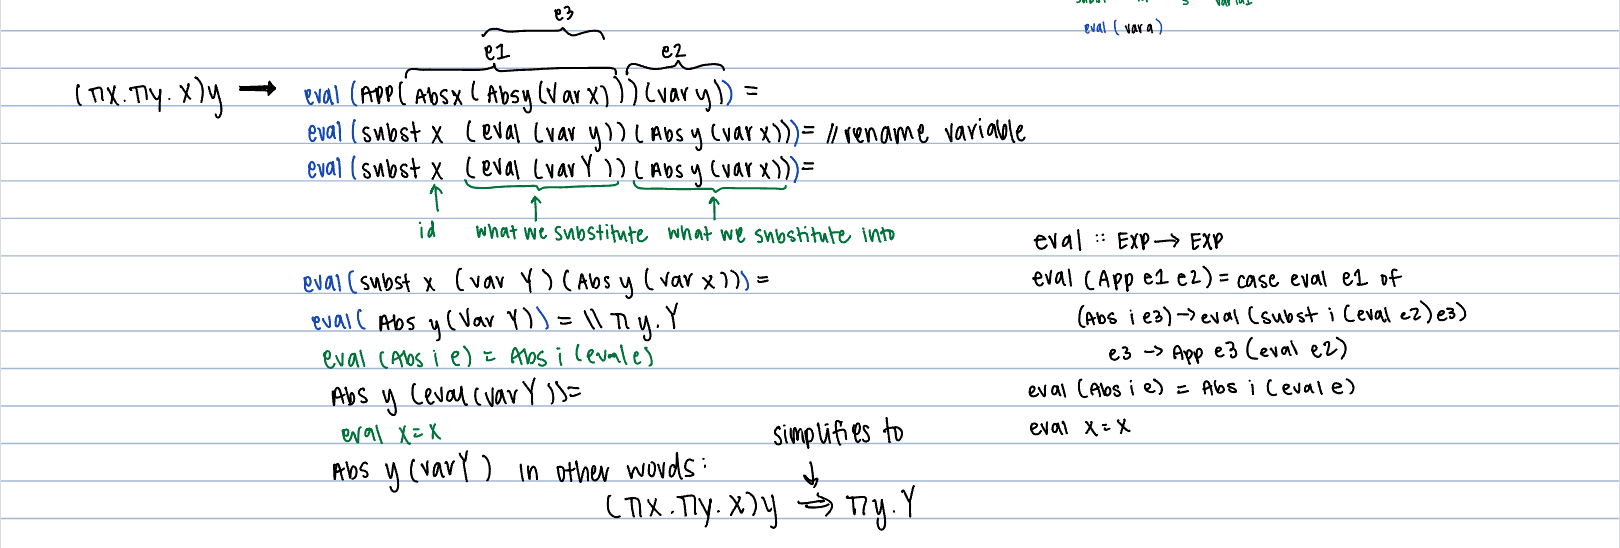
\includegraphics[width=15cm]{Week4hw_InClassProblem.jpg}
\end{center}

\subsection{Week 5}
For this week's homework we will review two main topics. The first is our discussion of variables, bindings, scope, and substition and the second is our practice of understanding the interpretation of lambda calculus. 
Before I include the excercises for the section, I will include a review of the terminology and concepts we discussed. To start, there are three types of variables we introduced; they are as follows:
\begin{itemize}
  \item fresh variable - a variables that has not been used before 
  \item bound variable - a variables that can be renamed by a fresh variable without changing the meaning
  \item free variable - a variable that is not bound and receives its meaning from the context in which it appears 
\end{itemize}
For example, in the expression \mintinline{haskell}{\x.x+y} the x is a bound variable and the y is a free variable. When we look at the scope of a variable, this simply means we have to take account the binding and paranthesis 
that apply to said variable. It's placement in the expression will affect the 
scope of the variable and therefore the meaning of it. This is a common topic in programming, especially as we turn to look at functions, classes, and their
respective variables. As a simple example, take the following function. 
\begin{center} 
  \begin{minted}{javascript}
      var f = function(a) {
        return a+3;     
    }
  \end{minted}
\end{center}
In the function defined above, the variable a only exists within the brackets of the function. Therefore, that is the scope of a. If a is referenced outside of its scope, an error will occur. Similarly, we can look at lambda calculus variables 
in the same way. The last term I will review is substitution. Substition is a common practice in mathematics, but it is important in lambda calculus as we begin to introduce the topic of capture avoiding substition. The reason we use CAS is to
prevent combining variables that may appear to be the same, but are not necessary equal. Therefore, the substition we will perform will avoid the ``capture" of these variables. Essentially, the idea is to look at the scope of the variables in the 
current expression and assess whether it is necessary to replace some of them with a fresh variable in order to dsitinguish the difference between itself and other variables in the following calculations. To see this in practice, I include the 
exercise provided for the homework below. \\


\textbf{Definition: } The function 
\begin{center}
  $f \circ g$
\end{center}
(pronounced "f after g") is the function obtained from taking the output of $g$ as the input of $f$. In the example, we want to replace the $x$ in $f(x) = x + y$ by 
$g(y) = y * 2$. It is tempting to write
\begin{center}
  $f \circ g(y) = f(g(y)) = 2 * y + y = 3y$
\end{center}
but this gives the \textbf{wrong} forumlformula for $f \circ g$. Such mistakes arise from not taking proper care of the distinction of free and bound variables. 
\begin{enumerate}
  \item What is the correct formula for the function $f \circ g$ in the example above?
  \item Use the notions of free and bound variables and score to explain your answer.
  \item Using lambda calculus write down a general formula for $f \circ g$ that works for abritrary f and g.
\end {enumerate}

Given the topic I have reviewed above, we can identify there is an issue in the above calculation regarding the variable $y$ and its scope. Although the $y$ variable in the functions $f$ and $g$ would be acceptable in many mathematical scenarios, this is 
not necessarily the case for us. Given that $y$ is a free variable in the function $f$ and a bound variable in the function $g$, we do not have enough information to ensure that they refer to the same value. It is possible that each $y$ is referring to 
a unique value. In other words, the binding to $y$ is not in the scope of the instance $y$ in the function $f$. Therefore, we cannot assume that it is bound to the same value. So, it is incorrect to simplify the expresion to $3y$. In order to correct this formula, 
we must use capture avoiding substitution. We can assign the $y$ in $f(x)$ a fresh variable to distinguish it from any other instances of $y$. The correct formula would therefore be: \\
\begin{center}
  $f(x) = x + Y$\\
  $g(y) = y * 2$

  \begin{align*}
    f \circ g(y) & = f(g(y)) \\
                & = 2 * y + Y \\
                & = 2y + Y
  \end{align*}
\end{center}
Since the $Y$ is a free variable it will remain in the solution as a variable. Meanwhile the bound $y$ will be substituted with a value if one is provided. As a general formula for $f \circ g$, we can represent it as: 
\begin{center}
  $f \circ g(y) = $ \mintinline{haskell}{\y.f(g(y))}
\end{center} 
As you can see, we do not include the $x$ variable in this formula because it is being replaced by the output of $g(y)$. If we assign a value to $f \circ g$ we will only have to pass in one value, that of $y$, so we do not need it in the formula. \\



Now, for the second half of this homework, we will switch into the discussion of the lambda calculator interpreter we have been using and gaining a deeper understanding into how and when the rules apply. This will also give us a better understanding of the topics we already 
mentioned such as variables, bindings, scope, and substitution. We were given the following task:\\

To understand how the interpreter works do the following.
\begin{itemize}
  \item Use Interpreter.hs to evaluate in the style above (equational reasoning as in Example 1 and 2) \begin{center}\mintinline{haskell}{(\x.\y.x)y}\end{center}Follow the implementation of eval and subst line by line, but choose your own fresh names to simplify the computation.
  \item For each variable appearing in subst say what its binder is and what the scope of the binder is.
\end{itemize}
Below I will include three pictures. The first is a simple screenshot of the Interpreter.hs file in order to understand what lines I am referring to in my computation. The second picture is a screenshot of the terminal output when the interpreter file is run with the input of the function above. 
The third picture is my handwritten computation of the equation \mintinline{haskell}{(\x.\y.x)y}. 
In my computation, the lines in grey represent my explanations or references to what is prompting the next step of computation. I also used different color parenthesis to avoid any misunderstanding of scopes of variables. Overall, the computation is quite simple. 
We must first evaluate the expression e1, which results in a recursive evaluation of both Abs cases in the expression. Once we have evaluated this, we can go back to the original expression and replace e1 for its evaluated value. Then, we can look at the definition of 
how to evaluation an App expression. This leads us to a substition. The reason this substitution is important is due to the fact that both $y$'s in the original expression are not necessarily equal in value. We must substitute one of them to avoid combining them. In this example, 
we substitute the \mintinline{haskell}{\y} for a reason. If we prioritize substitution this variable, we can easily replace the instances of $y$ it is binding. In this case, there are no $y$'s to replace in the body of the \mintinline{haskell}{\y.x} expression. Therefore, our 
result to this expression is \mintinline{haskell}{\A.y}. Since there are no $A$'s in the body of this, the expression would simply evaluate to \mintinline{haskell}{y}.

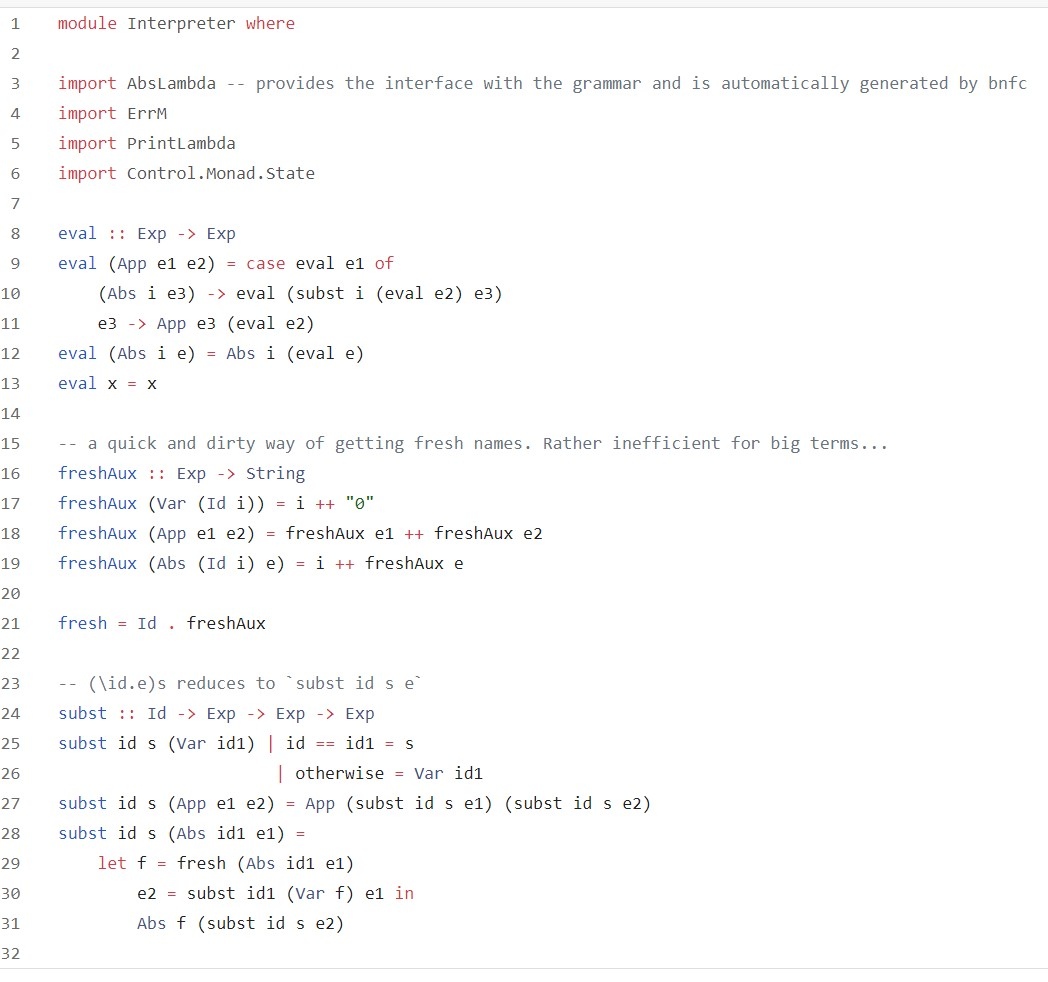
\includegraphics[width=15cm]{Week5hw_Interpreter.jpg}\\
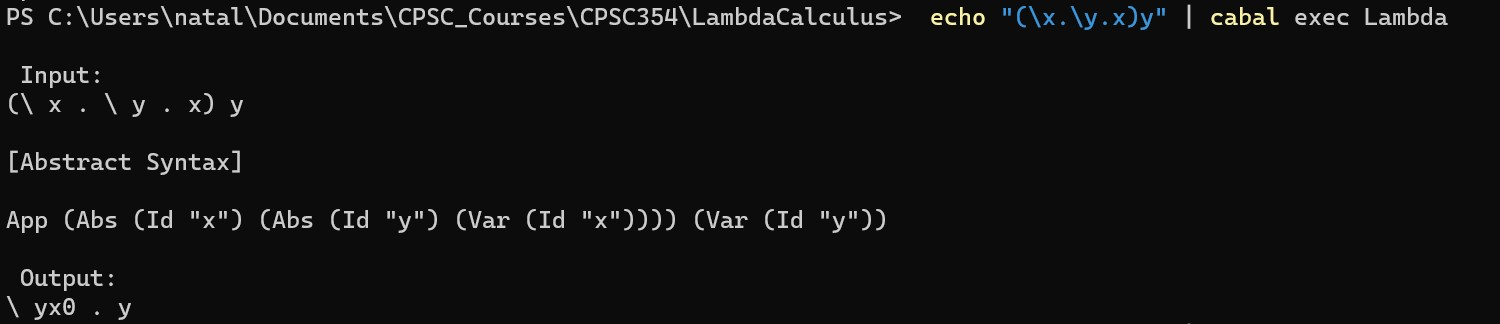
\includegraphics[width=15cm]{Week5hw_interpreterOutput.jpg}\\
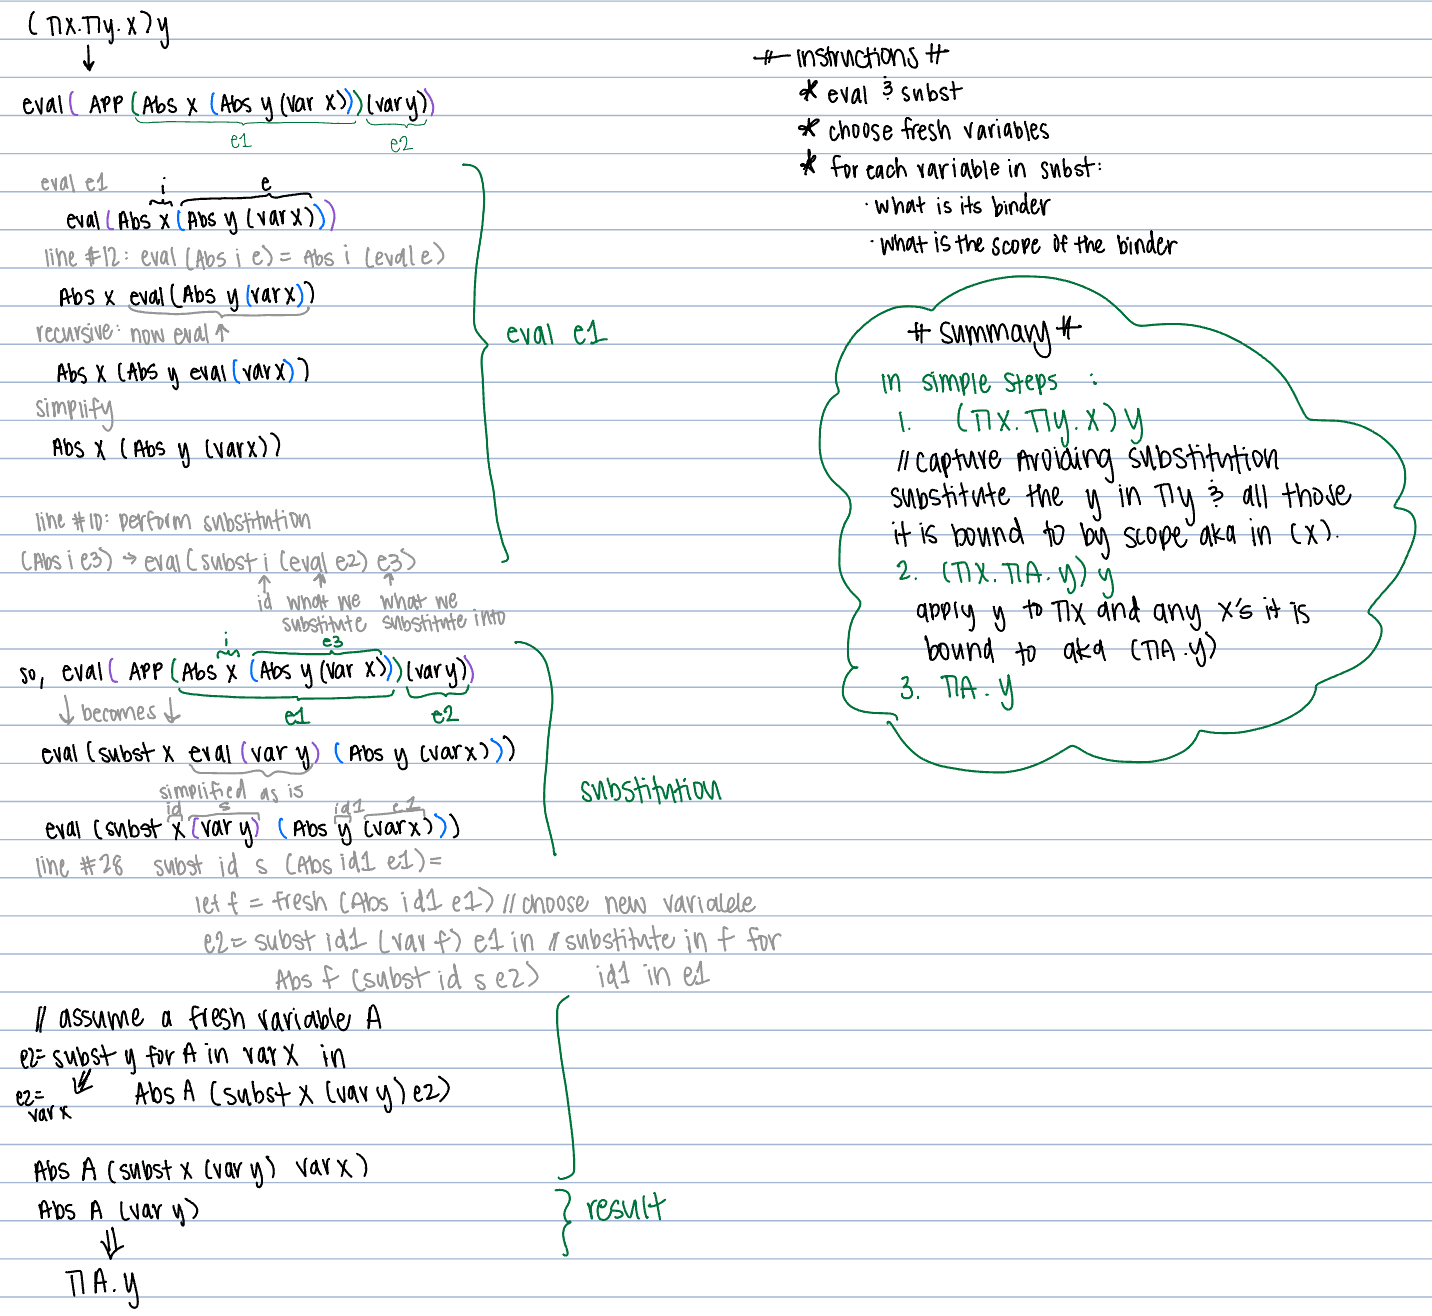
\includegraphics[width=15cm]{Week5hw_handwrittenInterpreter.jpg}

\subsection{Week 6}

The aim of this week's homework is to review what we learned in class about ARSs. An ARS, or an Abstraction Reduction System, provides you with rules that will allow you to reduce any expression composed of the letters in the given alphabet. I will first include the example we 
did in class and then include the excercises given to us as practice. 

So, the in-class example is as follows. Given the rewrite rules below, answer these questions:
\begin{center}
  \begin{minted}{haskell}
    aa -> a 
    bb -> a 
    ab -> b
    ba -> b 
  \end{minted}
\end{center}

\begin{itemize}
  \item \textbf{Why does the ARS terminate?}
    \begin{enumerate} 
      \item[] This ARS terminates when there is only one character left in the expression because this means there are no more rules that will shorten the string. 
      In other words, none of the given rewrite rules can be applied. Following this logic, there are three final outcomes that an expression can be simplified to. 
      These are `a', `b', and e. (Note: e stands for epsilon, which represents the empty string). The ARS cannot apply any of these rules to a single character or no character 
      because each rule being with a pair of letters. Each string will simplify to a single character because the rules account for every possible combiantion of a and b. 
    \end{enumerate}
  \item \textbf{What are the normal forms?} 
    \begin{enumerate} 
      \item[] The normal forms, or the strings that you cannot rewrite, are \mintinline{haskell}{a}, \mintinline{haskell}{b}, and \mintinline{haskell}{e}.
    \end{enumerate}
  \item \textbf{Is there a string \mintinline{haskell}{s} that reduces to both \mintinline{haskell}{a} and \mintinline{haskell}{b}?}
    \begin{enumerate} 
      \item[] There is not a string that reduces to both a and b. 
    \end{enumerate}
  \item \textbf{Show that the ARS is confluent.}
    \begin{enumerate} 
      \item[] An ARS is confluent if every "peak" contains a "valley". To test this, we will take the five cases of overlapping pairs, or the critical pairs, and compute whether these 
      two expressions will converge. In the picture below you can see how I tested these cases. The reason we want these to converge is because we want to see if they will all possible 
      routes will simplify to the same end result. So, we take each possible overlap and draw out the routes one could take to simplify it. In these cases, the left arrow points to the 
      string that results from applying the appropriate rewrite rule to the left-most pair of letters in the original string and copying over the last letter. The right arrow points to
      the string that reults from copying over the first letter and applying the appropriate rewrite rule to the right-most pair of letters. We can see that in every case, the different 
      routes of computation converge to the same end string. Therefore, we can say that this ARS is confluent. \\
      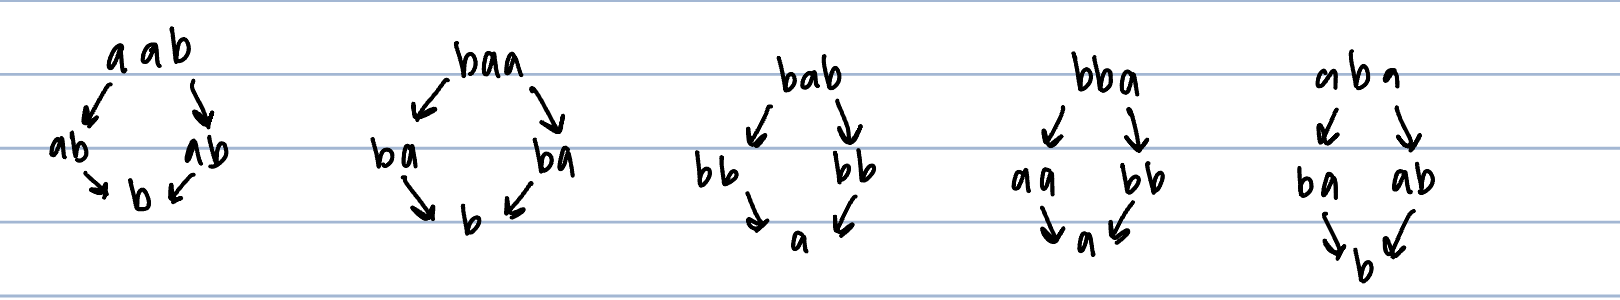
\includegraphics[width=12cm]{confluent.png}\\
    \end{enumerate}
  \item \textbf{Replacing \mintinline{haskell}{->} by \mintinline{haskell}{=}, which words become equal?}
    \begin{enumerate} 
      \item[] If we replace \mintinline{haskell}{->} by \mintinline{haskell}{=}, then all words that simply to \mintinline{haskell}{a} become equal and all words that simplify to 
      \mintinline{haskell}{b} become equal. Logically, this makes sense because if two strings simplify to the same letter, then the rewrite rules can be used backwards to result in either 
      string. As we discussed this question and as I tested many cases to understand the nature of the rules, we also discovered that if a string contains an odd number of \mintinline{haskell}{b}s its 
      normal form is \mintinline{haskell}{b} and if a string contains an even number of \mintinline{haskell}{b}s then its normal form is \mintinline{haskell}{a}.
    \end{enumerate}
\end{itemize}



Now having reviewed the in-class example, we will look at the assigned exercises. First we are prompted to draw a picture for each of the following ARSs:
\begin{enumerate}
  \item \mintinline{haskell}{A = {}}
  \item \mintinline{haskell}{A = {a} , R = {}}
  \item \mintinline{haskell}{A = {a} , R = {(a,a)}}
  \item \mintinline{haskell}{A = {a, b, c} , R = {(a, b), (a, c)}}
  \item \mintinline{haskell}{A = {a, b} , R = {(a, a), (a, b)}}
  \item \mintinline{haskell}{A = {a, b, c} , R = {(a, b), (b, b), (a, c)}}
  \item \mintinline{haskell}{A = {a, b, c} , R = {(a, b), (b, b), (a, c), (c, c)}}
\end{enumerate}

\includegraphics[width=15cm]{arsDrawn.png}

Lastly, we will find an example ARS for each of the following combinations in the table. I include my solution as a screenshot from my digital handwritten notes. 
\begin{center}
  \begin{tabular}{||c c c ||} 
   \hline
   confluent & terminating & unique normal forms \\ [0.5ex] 
   \hline\hline
   true & true & true \\ 
   \hline
   true & true & false \\
   \hline
   true & false & true \\
   \hline
   true & false & false \\
   \hline
   false & true & true \\
   \hline
   false & true & false \\
   \hline
   false & false & true \\
   \hline
   false & false & false \\ [1ex] 
   \hline
  \end{tabular}
\end{center}
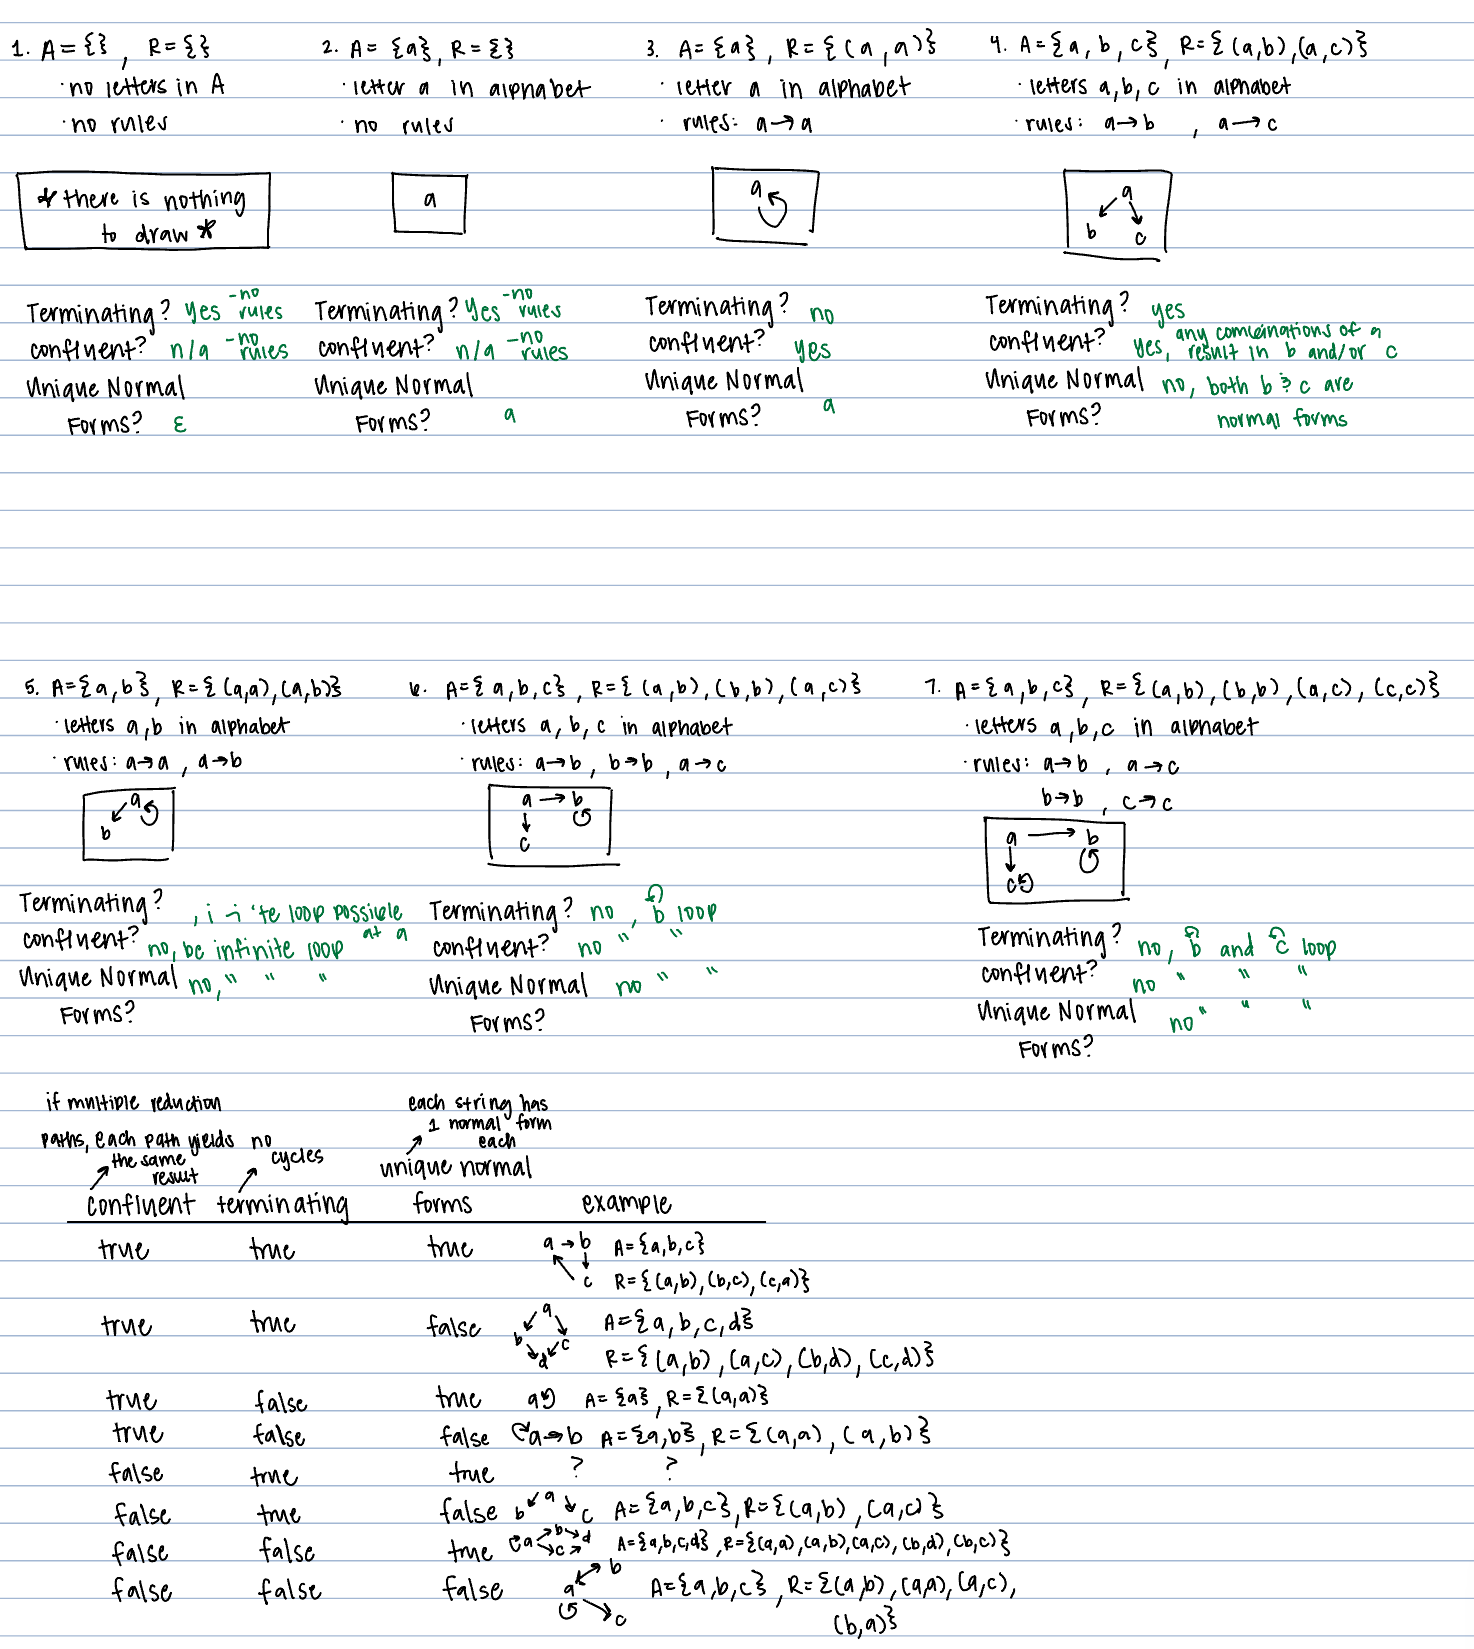
\includegraphics[width=15cm]{arsTable.png}

EDIT: I add this note after having gone over a few of the examples above during our lecture. One of the main ideas we discussed was whether we could say that any of the three properties (that is: confluence, termination, and unique normal forms[UNF]) 
implies the others. We were ultimately able to agree upon the idea that if an ARS is both confluent and terminating then this implies it has UNFs. The confluence gives the ARS its uniqueness given that all "peaks" have a "valley" that lead it to the same 
end result. The termination of the ARS means it has normal forms. So, together they imply the existence of unique normal forms for the ARS. Having this new understading of the relationships of these three properties, we can look back at my notes and 
note that some of my examples are incorrect. Specifically, the row that describes an ARS that is confluent and terminating but does not have UNFs. This is not possible since the first two imply the last property. From my understanding
this would also mean that when either of the first two are false, the UNFs property must be false as well. I include an edited version of my notes below.
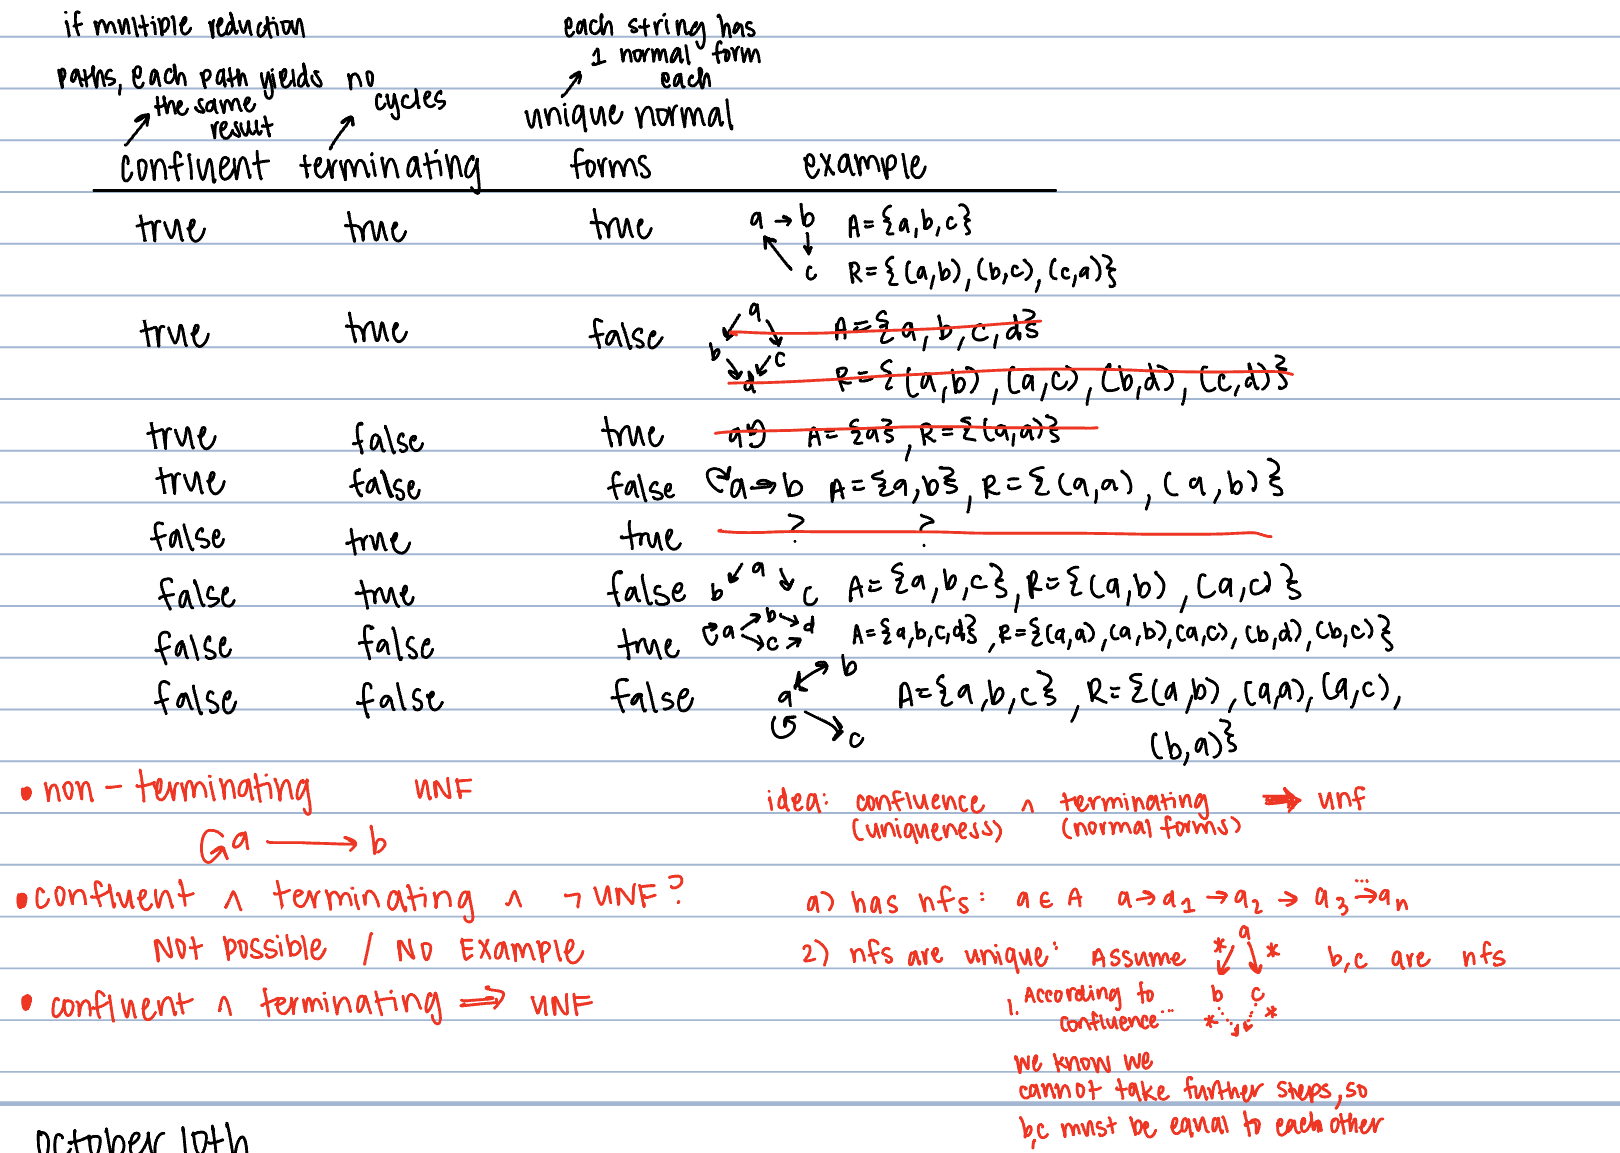
\includegraphics[width=15cm]{arsTableEdit.png}

\subsection{Week 7}
For this week's homework we are reviewing what we learned about invariants. An invariant is a property we can identify that remains unchanged regardless of the input or the operations performed. An easy example for an invariant is to think of a mathematical 
formula that we commonly use. The area of a rectangle or the conversion from Fahrenheit to Celsius are two examples. Regardless of the measurements given to you, the formula of an area of a rectangle will always hold true and will not change. So, this relationship
or this formula is an invariant. Now, we can use invariants to prove or disprove scenarios. If we can prove that an invariant does not apply to a case, then that case should be false. \\

In class, we looked at the chessboard puzzle and used the invariant of how many white squares there were compared to black squares based on which tiles were removed. For this homework, I will look at one of the puzzles we did not discuss in class, but 
that was included as an example of a puzzle we could discuss, the Tetris Puzzle. I include the description of the puzzle in the below image. \\

\begin{center}
  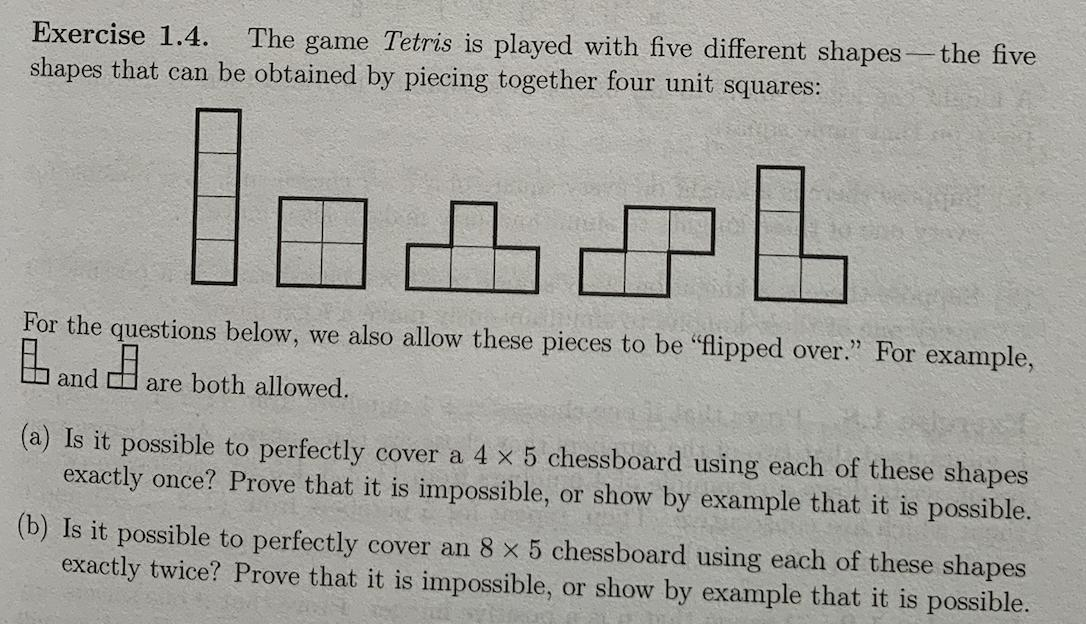
\includegraphics[width=10cm]{tetrisDesc.jpg}
\end{center}

I stared at this problem for a while, trying to figure out a way to determine if I could fill the board with some sort of formula or invariant. After multiple failed attempts, I thought it was impossible to find a configuration that would successfully cover the 
4x5 board with the tetris tiles. The number of tiles of the five tetrinomes was equal to the number of tiles on the board, 20. However, they weren't fitting together in a way that would be acceptable. So, I looked back at our in-class example, the chessboard 
puzzle, and decided to use a similar approach. If we color the 4x5 with alternating colors, just like a chessboard, and the 5 tetrinomes as well, we can make an interesting observation. The board results in 20 total tiles, so 10 white tiles and 10 black tiles. 
The tetrinomes result in either 11 black tiles and 9 white tiles or 9 black tiles and 11 white tiles depending on where the alternations colors begin. In each case, the number of black and white tiles is unequal to the those on the 4x5 grid. If we look at it this way, 
we can reason that there is not possible configuration for the tetrinomes to cover the grid completely. The invariant here would that the number of black tiles - the number of white tiles needs to equal zero. Here, this formula would equal 2 or -2, not zero. I include 
my drawing of the tetrinomes and grid with alternating colors below. \\

\begin{center}
  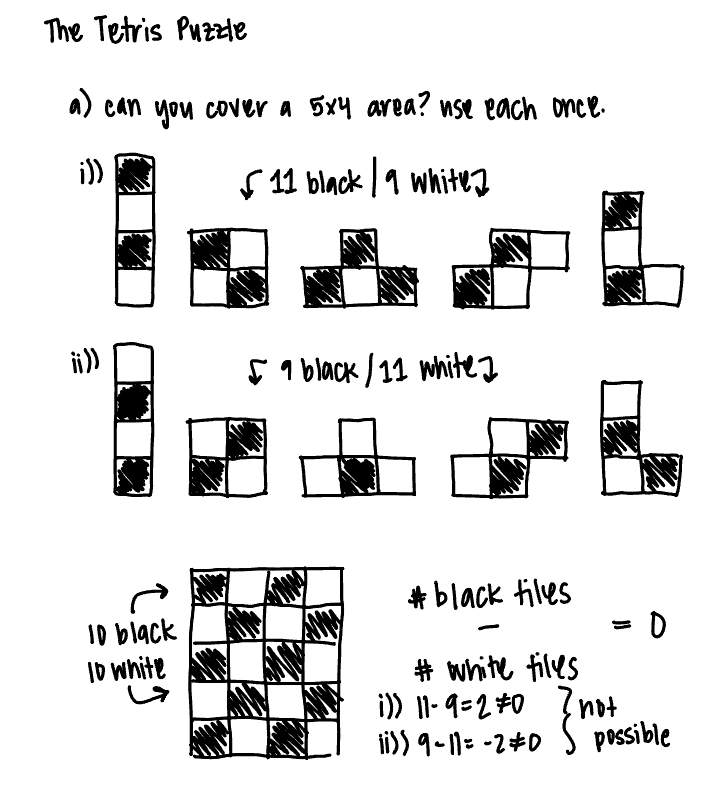
\includegraphics[width=9cm]{tetrisA.png}
\end{center}

Now that we have discussed part a, part b is asking us if we can cover an 8x5 board by using each of the tetrinomes exactly twice. Let's use the same logic here. Again, the tiles and their colors remain the same and board simply expands. 
If we are using each tetrinome exactly twice, this means we have three possible combinations of colored tiles. The only tetrinome that affects this is the T shape so lets focus on this. We can have two T's with more black tiles each, two T's with more white tiles each, or 
two T's, one with more black tiles and the other with more white tiles. This leaves us with three possible combinations of total colored tiles. \\

\begin{itemize}
  \item 1. 22 black tiles, 18 white tiles 
  \item 2. 18 black tiles, 22 white tiles 
  \item 3. 20 black tiles, 20 white tiles
\end{itemize}

The first two cases, of course, indicate it is not possible to cover the 8x5 grid with those particular combinations of tiles. However, the third case does match that of the grid, so we can say that there is a configuration that will allow us to cover the 8x5 grid with that 
combination of tiles. The two T tiles in thise scenario are opposite of one another, so their uneven number of alternating colors cancel out here. The invariant, again, here also proves this because 22-18 and 18-22 are not equal to zero but 20-20 is equal to zero. Below, I include 
again my drawings of the tiles and the configuration I found to satisfy the puzzle using my knowledge of the invariant. \\

\begin{center}
  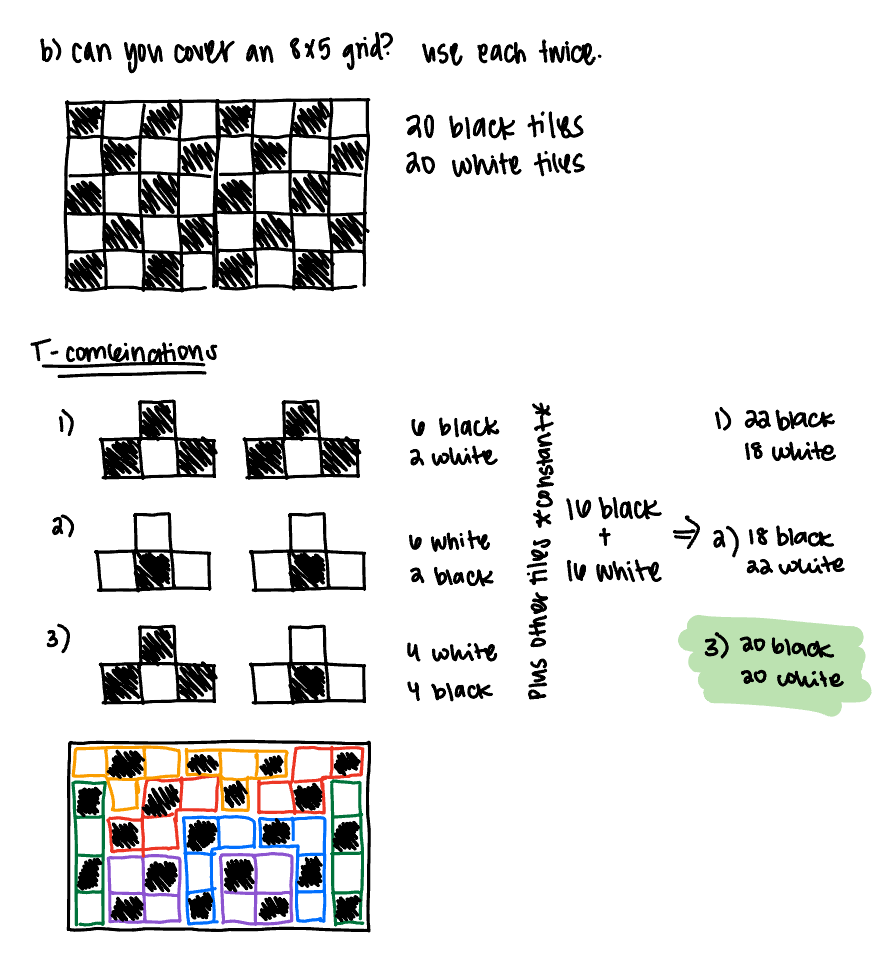
\includegraphics[width=9cm]{tetrisB.png}
\end{center}

By using invariants, we can go about proving or disproving questions more efficiently rather than trying to plug in values until we can find a set that is satisfactory or until we notice the pattern. It allows us to apply our mathematical foundations and definitions to other areas, 
such as computer science. 


\subsection{Week 10}

FIXME: EXPLAIN WHAT THE ASSIGNMENT WAS - PRISONER'S DILEMMA I THINK - AND WHAT TF ARE YOU TALKING ABOUT BELOW 

When a player clicks on the “send blocks” button, this post request is executed. I will describe step-by-step what occurs based on my understanding using the debugger for this assignment. 

The server will first receive the request to execute the endpoint and receive both the player’s code and the player’s ID. It will then check if both players have submitted their code. If they have, the server will try to run the game using the runGame(playerCodes[0], playerCodes[1]) function. 
The result of the game will then be sent to the client. If both players have not submitted their code, the server will wait for 10 seconds for the other player to respond with their code. At each second, it will check if the second player has submitted their code and the game has finished. If 
so, the game result will be sent to the client. If in the 10 seconds, there is no detection of the second player’s response, then the server will indicate it did not receive it. 

For both players to get the result of the game, both must submit their code relatively close to each other. In this case, it would need to be within 10 seconds of each other because that is how long the loop will keep checking for both responses. Otherwise, it is possible that only the second 
player gets the result. This is possible because the first player will stop checking for the second player’s code and will therefore not get the result of the game. The second player, however, when submitting its code will prompt the runGame function and then get the result once it completes. 
To fix this, I would consider changing the 10 second timeout on the loop checking for the second player’s code. Otherwise, this situation will continue to be possible. 

Using a debugger is helpful because it allows you to step through the code and see the changes in variables and the flow of function calls line by line. I had some issues using the debugger in that it stopped working suddenly and I have not been able to find a solution yet, but I plan to keep
 testing it and trying to fix it so I can use it for future projects and assignments. 

Additionally, I did use AI for this assignment to understand the code a bit better, but all that was written above is my own work. 


\subsection{Lesson From the Project}

FIXME: (5 PAGES)
- WHAT IS THE PROJECT, WHAT WAS ITS PURPOSE 
- GIVE A DESCRIPTION OF WHAT I CONTRIBUTED AND WHERE WE CAN FIND THE PROJECT 
- WHAT WAS OUR GOAL AND WHAT DID WE ACTUALY ACHIEVE 
- WHAT ARE THE TECHNICAL SKILLS I LEARNED 
- WHAT ARE THE NON-TECHNICAL SKILLS I LEARNED 
- WHAT DID I LEARN FROM THE LECTURES AND THE REPORT AND HOW DID THEY CONTRIBUTE TO THE PROJECT OR TO OTHER CLASSES/WORK 
- CAN I RELATE THIS TO ALGORITHM ANALYSIS CLASS PERHAPS 
- DO I HAVE ANY REFLECTIONS FRROM THE PROJECT AS A WHOLE 
- REMAINING OR LINGERING QUESTIONS, COMMENTS, OR OBSERVATIONS ABOUT THE PROJECT AND ABOUT THE CLASS 
- WHAT DID I STRUGGLE WITH THE MOST MAYBE 

\ldots

\section{Conclusions}\label{conclusions}

(approx 400 words) A critical reflection on the content of the course. Step back from the technical details. How does the course fit into the wider world of software engineering? What did you find most interesting or useful? 
What improvements would you suggest?

\begin{thebibliography}{99}
\bibitem[ALG]{Alg} \href{https://github.com/alexhkurz/algorithm-analysis-2023}{Algorithm Analysis}, Chapman University, 2023.
\end{thebibliography}

\end{document}